\section{Filip Kowalski}
\label{sec:fk}

Dodałem zdjęcie pandy (zobacz Rysunek~\ref{fk:fig:plush_panda}).

\begin{figure}[htbp]
    \centering
    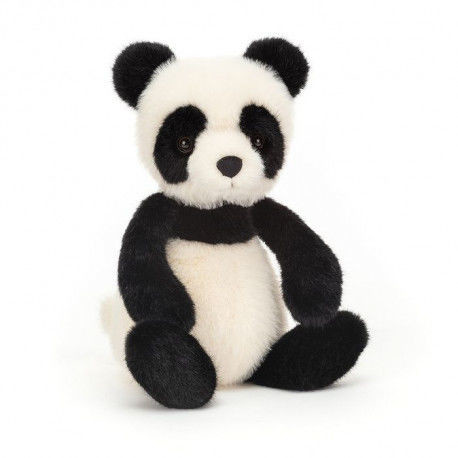
\includegraphics[width=0.2\textwidth]{pictures/plush_panda.jpg} % Jak sprawić, żeby obrazek był większy?
    \caption{Pog panda}
    \label{fk:fig:plush_panda}
\end{figure}

Tabela~\ref{fk:tab:ptaki} przedstawia całkowitą ilość zgonów i występowanie ptaków na poszczególnych planetach Układu Słonecznego. Łatwo zauważyć, że występowanie ptaków jest \textbf{ściśle powiązane} jest z ogromną ilością zgonów.

% Please add the following required packages to your document preamble:
% \usepackage[table,xcdraw]{xcolor}
% If you use beamer only pass "xcolor=table" option, i.e. \documentclass[xcolor=table]{beamer}
\begin{table}[h]
\begin{tabular}{|r|c|c|}
\hline
\rowcolor[HTML]{FFFFC7} 
\multicolumn{1}{|l|}{\cellcolor[HTML]{FFFFC7}Planeta} &
  \multicolumn{1}{l|}{\cellcolor[HTML]{FFFFC7}Ilość zgonów} &
  \multicolumn{1}{l|}{\cellcolor[HTML]{FFFFC7}Występowanie ptaków} \\ \hline\hline
Merkury         & 0                           & Nie          \\ \hline
Wenus           & 0                           & Nie          \\ \hline
\textbf{Ziemia} & \textbf{>120,000,000,000} & \textbf{Tak} \\ \hline
Mars            & 0                           & Nie          \\ \hline
Jowisz          & 0                           & Nie          \\ \hline
Saturn          & 0                           & Nie          \\ \hline
Uran            & 0                           & Nie          \\ \hline
Neptun          & 0                           & Nie          \\ \hline
Pluton          & 0                           & Nie          \\ \hline
\end{tabular}
 \centering
\label{fk:tab:ptaki}
\caption{Ptaki instrumentem zagłady i zniszczenia wszelkiego życia na Ziemii}
\end{table}

Energię elektonu w atomie można wyznaczyć korzystając ze wzoru:

$$ E = -\frac{m_e e^4}{8\varepsilon^2h^2n^2}$$

gdzie:

\begin{itemize}
  \item[-] $m_e$ to masa elektronu,
  \item[-] $e$ to ładunek elektronu,
  \item[-] $\varepsilon$ to przenikalność elektryczna próżni,
  \item[-] {\it n} to główna liczba kwantowa.
\end{itemize}

\newpage

\begin{flushleft}
Top 10 natural numbers:
\begin{etaremune}
  \item Wszystkie
  \item liczby
  \item naturalne
  \item są spoko
  \item nie
  \item można
  \item ustawić
  \item ich
  \item w rankingu
  \item 69
\end{etaremune}
\end{flushleft}

\vspace{2em}

\begin{center}
    W sumie to \textbf{nie} wiem co \textit{tu} napisać \par
    Lorem ipsum, \underline{dolor} sit \textbf{\textit{\underline{amet}}}.
\end{center}